\newcommand{\flooderTagResultsAucTable}{
    \begin{table}[H]
        \centering
        \begin{tabular}{|p{2,8cm}||p{2,8cm} p{2,8cm} p{2,8cm}|}
            \hline
            Flooder Tag & ALOHA & Joint Embedding & Proposed Model \\
            \hline
            AUC-ROC & \textBF{0.596$\pm$0.108} & 0.390$\pm$0.206 & 0.564$\pm$0.110 \\
            \hline
        \end{tabular}
        \caption{AUC-ROC (Area Under Curve) of the different models for the \textbf{Flooder Tag} prediction task. Results were aggregated over \textBF{3} training runs with different weight initializations and minibatch orderings. Best results are shown in \textbf{bold}.} \label{tab:flooderTag_auc}
    \end{table}
}

\newcommand{\flooderTagResultsAtFprTable}{
    \begin{center}
        \begin{longtable}[c]{|p{3,2cm}||p{1,8cm} p{1,8cm} p{1,8cm} p{1,8cm} p{1,8cm}|}
            \hline
            Flooder Tag & \multicolumn{5}{c|}{{FPR}} \\
            & $10^{-5}$ & $10^{-4}$ & $10^{-3}$ & $10^{-2}$ & $10^{-1}$ \\
            \hline
            \endfirsthead

            \caption*{\raggedright ...continued from previous page} \\
            \hline
            Flooder Tag & \multicolumn{5}{c|}{\textbf{FPR}} \\
            & $10^{-5}$ & $10^{-4}$ & $10^{-3}$ & $10^{-2}$ & $10^{-1}$ \\
            \hline
            \endhead

            \caption*{\raggedleft ...continued on next page} \\
            \endfoot

            \caption{Mean and standard deviation results (TPR, Accuracy, Recall, Precision and F1-Score) of the different models for the \textbf{Flooder Tag} prediction task at different \textbf{FPR}s (\textit{False Positive Rates}). Results were aggregated over \textBF{3} training runs with different weight initializations and minibatch orderings. Best results are shown in \textbf{bold}. Under \textbf{TPR} results are also presented the percentage reduction in mean detection error and in ROC curve standard deviation introduced by the \textit{Proposed Model} with respect to both \textit{ALOHA} model and \textit{Joint Embedding}.} \label{tab:flooderTag_results_at_fpr} \\
            \endlastfoot

            \multicolumn{6}{|c|}{\textbf{TPR}} \\
            \hline
            ALOHA & \textBF{0.000$\pm$0.000} & \textBF{0.000$\pm$0.000} & \textBF{0.000$\pm$0.000} & \textBF{0.000$\pm$0.000} & 0.111$\pm$0.157 \\
            Joint Embedding & \textBF{0.000$\pm$0.000} & \textBF{0.000$\pm$0.000} & \textBF{0.000$\pm$0.000} & \textBF{0.000$\pm$0.000} & \textBF{0.222$\pm$0.314} \\
            Proposed Model & \textBF{0.000$\pm$0.000} & \textBF{0.000$\pm$0.000} & \textBF{0.000$\pm$0.000} & \textBF{0.000$\pm$0.000} & 0.000$\pm$0.000 \\
            \hline
            Error Reduction wrt \newline ALOHA & 0.0\% & 0.0\% & 0.0\% & 0.0\% & -12.5\% \\
            Error Reduction wrt \newline Joint Embedding & 0.0\% & 0.0\% & 0.0\% & 0.0\% & -28.5\% \\
            \hline
            Std Reduction wrt \newline ALOHA & 0.0\% & 0.0\% & 0.0\% & 0.0\% & 100.0\% \\
            Std Reduction wrt \newline Joint Embedding & 0.0\% & 0.0\% & 0.0\% & 0.0\% & 100.0\% \\
            \hline
            \multicolumn{6}{|c|}{\textbf{Accuracy}} \\
            \hline
            ALOHA & \textBF{0.999$\pm$0.000} & \textBF{0.999$\pm$0.000} & \textBF{0.998$\pm$0.000} & \textBF{0.998$\pm$0.000} & 0.962$\pm$0.041 \\
            Joint Embedding & \textBF{0.999$\pm$0.000} & \textBF{0.999$\pm$0.000} & \textBF{0.998$\pm$0.000} & 0.998$\pm$0.001 & 0.973$\pm$0.034 \\
            Proposed Model & \textBF{0.999$\pm$0.000} & \textBF{0.999$\pm$0.000} & \textBF{0.998$\pm$0.000} & \textBF{0.998$\pm$0.000} & \textBF{0.983$\pm$0.014} \\
            \hline
            \multicolumn{6}{|c|}{\textbf{Recall}} \\
            \hline
            ALOHA & \textBF{0.000$\pm$0.000} & \textBF{0.000$\pm$0.000} & \textBF{0.000$\pm$0.000} & \textBF{0.000$\pm$0.000} & 0.111$\pm$0.157 \\
            Joint Embedding & \textBF{0.000$\pm$0.000} & \textBF{0.000$\pm$0.000} & \textBF{0.000$\pm$0.000} & \textBF{0.000$\pm$0.000} & \textBF{0.222$\pm$0.314} \\
            Proposed Model & \textBF{0.000$\pm$0.000} & \textBF{0.000$\pm$0.000} & \textBF{0.000$\pm$0.000} & \textBF{0.000$\pm$0.000} & 0.000$\pm$0.000 \\
            \hline
            \multicolumn{6}{|c|}{\textbf{Precision}} \\
            \hline
            ALOHA & \textBF{1.000$\pm$0.000} & \textBF{1.000$\pm$0.000} & \textBF{0.000$\pm$0.000} & \textBF{0.000$\pm$0.000} & 0.001$\pm$0.002 \\
            Joint Embedding & \textBF{1.000$\pm$0.000} & \textBF{1.000$\pm$0.000} & \textBF{0.000$\pm$0.000} & \textBF{0.000$\pm$0.000} & \textBF{0.004$\pm$0.005} \\
            Proposed Model & \textBF{1.000$\pm$0.000} & \textBF{1.000$\pm$0.000} & \textBF{0.000$\pm$0.000} & \textBF{0.000$\pm$0.000} & 0.000$\pm$0.000 \\
            \hline
            \multicolumn{6}{|c|}{\textbf{F1 Score}} \\
            \hline
            ALOHA & \textBF{0.000$\pm$0.000} & \textBF{0.000$\pm$0.000} & \textBF{0.000$\pm$0.000} & \textBF{0.000$\pm$0.000} & 0.003$\pm$0.004 \\
            Joint Embedding & \textBF{0.000$\pm$0.000} & \textBF{0.000$\pm$0.000} & \textBF{0.000$\pm$0.000} & \textBF{0.000$\pm$0.000} & \textBF{0.007$\pm$0.010} \\
            Proposed Model & \textBF{0.000$\pm$0.000} & \textBF{0.000$\pm$0.000} & \textBF{0.000$\pm$0.000} & \textBF{0.000$\pm$0.000} & 0.000$\pm$0.000 \\
            \hline
        \end{longtable}
    \end{center}
}

\newcommand{\flooderTagResultsSummaryTable}{
    \begin{table}[H]
        \centering
        \begin{tabular}{|p{3,2cm}||p{1,8cm} p{1,8cm} p{1,8cm} p{1,8cm} p{1,8cm}|}
            \hline
            \multicolumn{6}{|c|}{Flooder Tag (at FPR $=1\%$)} \\
            \hline
            Model & TPR & Accuracy & Precision & Recall & F1 score \\
            \hline
            ALOHA & \textBF{0.000$\pm$0.000} & \textBF{0.998$\pm$0.000} & \textBF{0.000$\pm$0.000} & \textBF{0.000$\pm$0.000} & \textBF{0.000$\pm$0.000} \\
            Joint Embedding & \textBF{0.000$\pm$0.000} & 0.998$\pm$0.001 & \textBF{0.000$\pm$0.000} & \textBF{0.000$\pm$0.000} & \textBF{0.000$\pm$0.000} \\
            Proposed Model & \textBF{0.000$\pm$0.000} & \textBF{0.998$\pm$0.000} & \textBF{0.000$\pm$0.000} & \textBF{0.000$\pm$0.000} & \textBF{0.000$\pm$0.000} \\
            \hline
        \end{tabular}
        \caption{Summary of the mean and standard deviation results of the different models for the \textbf{Flooder Tag} prediction task at \textbf{FPR} $=1\%$. Results were aggregated over \textBF{3} training runs with different weight initializations and minibatch orderings. Best results are shown in \textbf{bold}.} \label{tab:flooderTag_result_summary}
    \end{table}
}

\newcommand{\flooderTagRocAloha}{
    \begin{figure}[H]
        \centering
        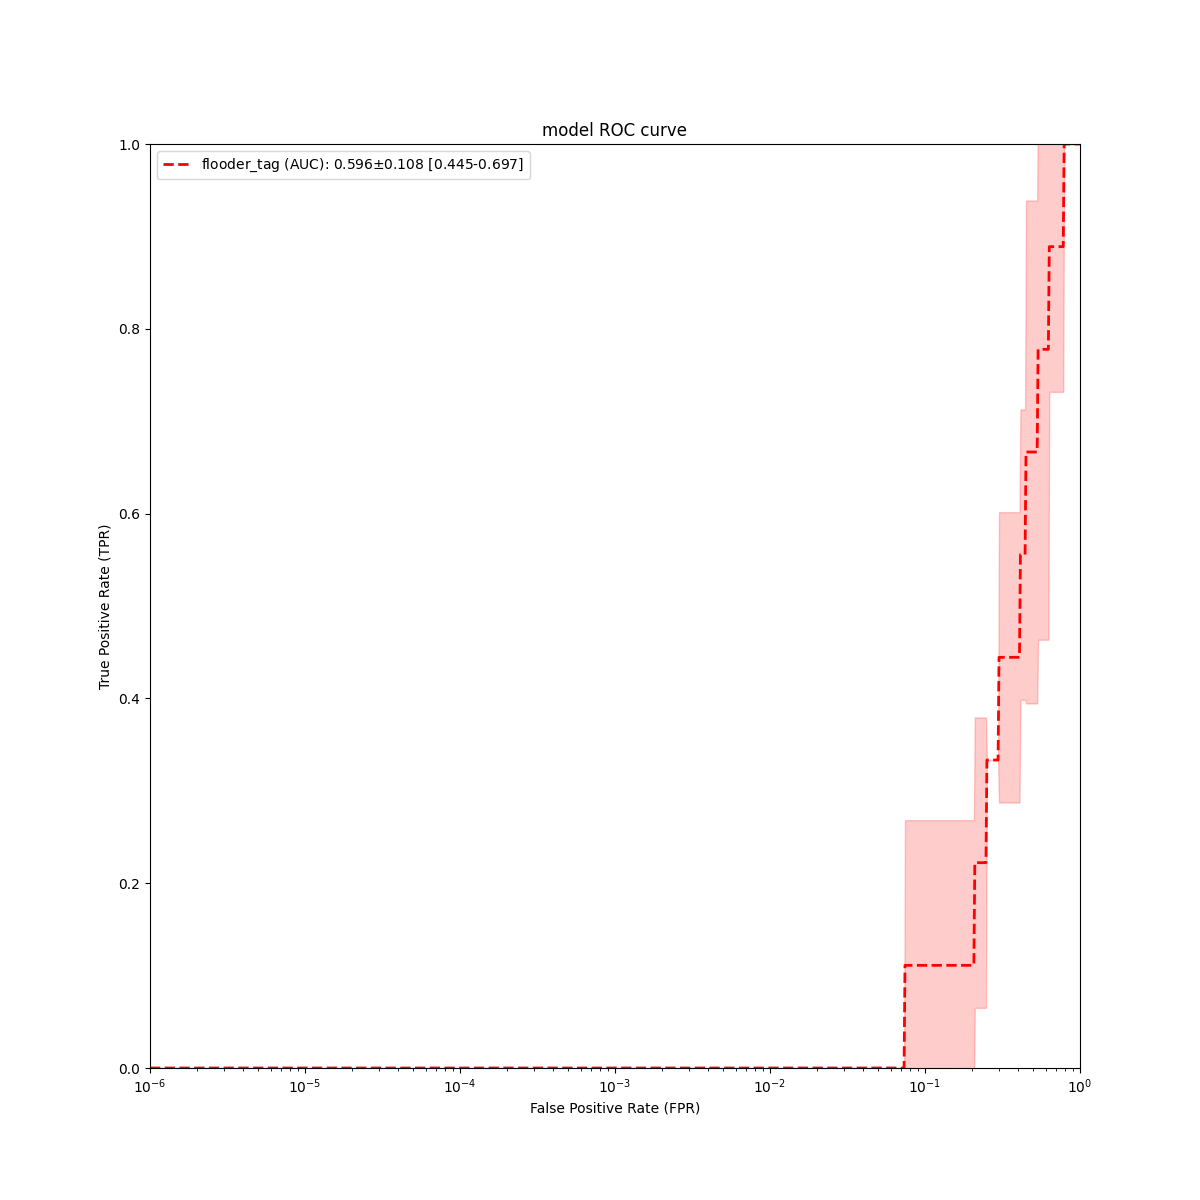
\includegraphics[width=0.8\textwidth]{./results/flooder_tag_roc_aloha.png}
        \vspace*{-1cm}
        \caption{ROC curve and AUC statistics of \textBF{ALOHA} model for the \textbf{Flooder Tag}. The line represents the \textit{mean} TPR at a given FPR, while the shaded region represents the \textit{standard deviation}. Statistics were computed over \textBF{3} training runs, each with random parameter initialization.}
        \label{fig:flooderTagRocAloha}
    \end{figure}
}

\newcommand{\flooderTagRocJointEmbedding}{
    \begin{figure}[H]
        \centering
        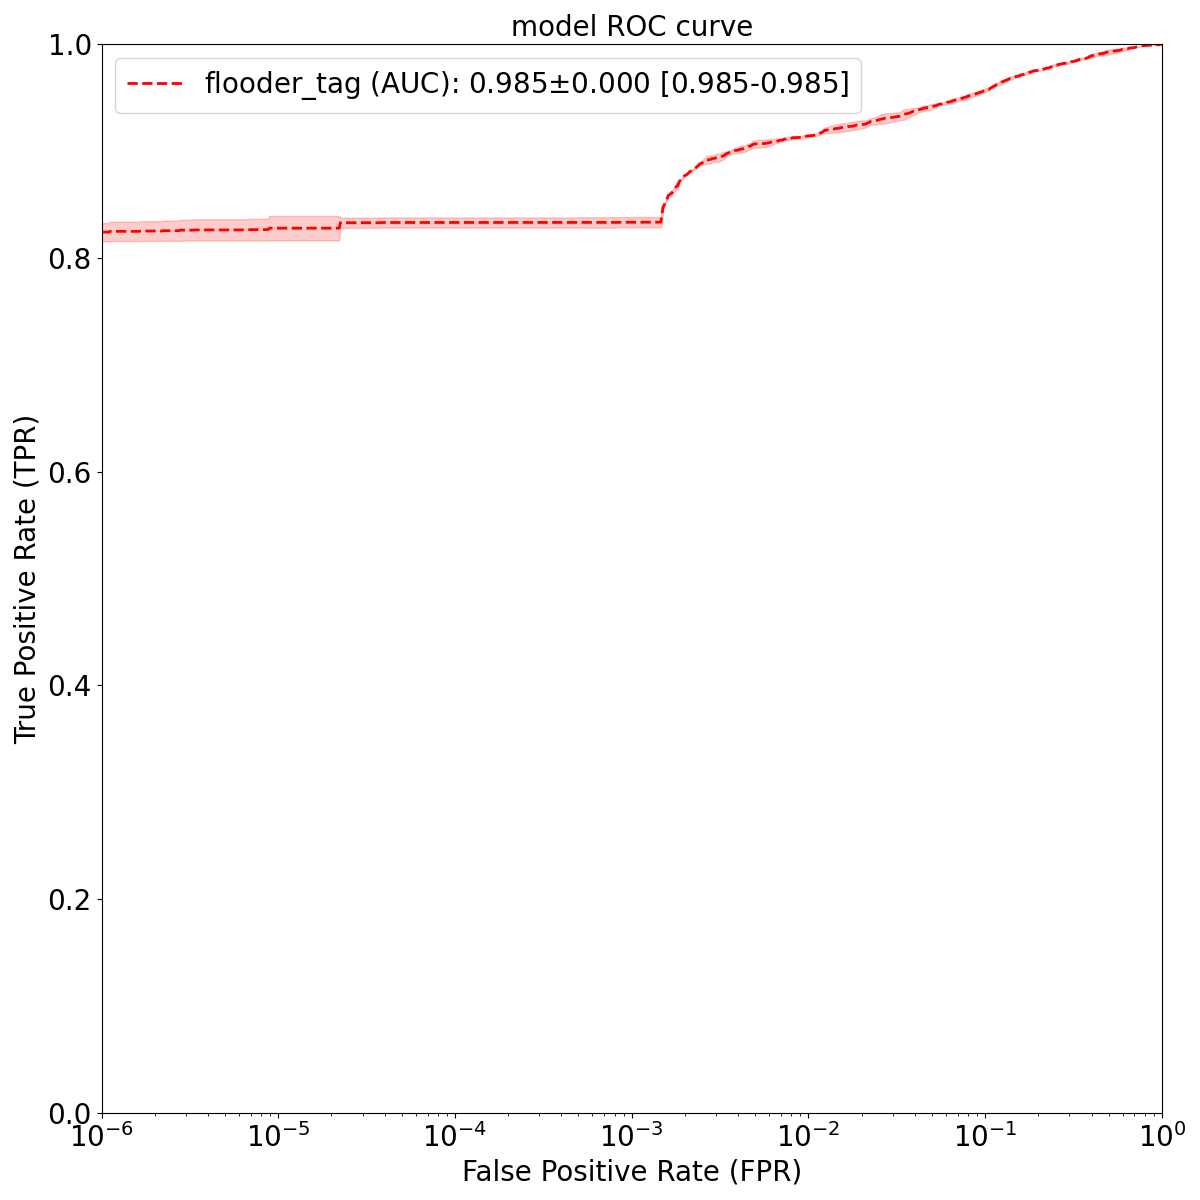
\includegraphics[width=0.8\textwidth]{./results/flooder_tag_roc_jointEmbedding.png}
        \vspace*{-1cm}
        \caption{ROC curve and AUC statistics of \textBF{Joint Embedding} model for the \textbf{Flooder Tag}. The line represents the \textit{mean} TPR at a given FPR, while the shaded region represents the \textit{standard deviation}. Statistics were computed over \textBF{3} training runs, each with random parameter initialization.}
        \label{fig:flooderTagRocJointEmbedding}
    \end{figure}
}

\newcommand{\flooderTagRocProposedMethod}{
    \begin{figure}[H]
        \centering
        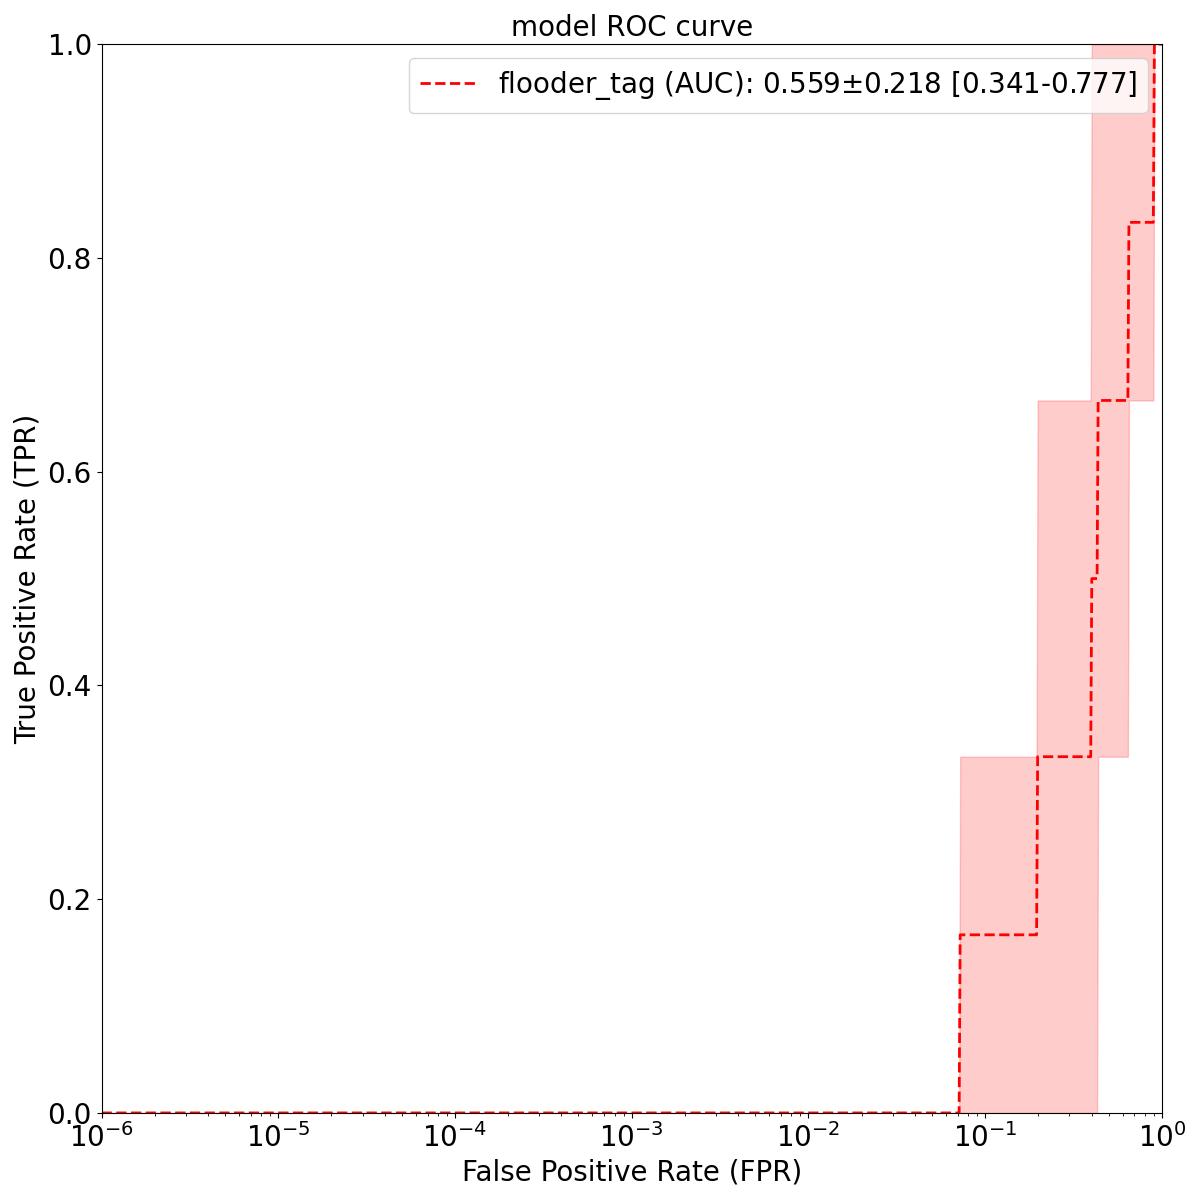
\includegraphics[width=0.8\textwidth]{./results/flooder_tag_roc_proposedModel.png}
        \vspace*{-1cm}
        \caption{ROC curve and AUC statistics of \textBF{Proposed Model} for the \textbf{Flooder Tag}. The line represents the \textit{mean} TPR at a given FPR, while the shaded region represents the \textit{standard deviation}. Statistics were computed over \textBF{3} training runs, each with random parameter initialization.}
        \label{fig:flooderTagRocProposedModel}
    \end{figure}
}
